\documentclass{article}
\usepackage[papersize={214mm,160mm},tmargin=10mm, 
bmargin=10mm,lmargin=10mm, rmargin=10mm]{geometry}

\usepackage[utf8]{inputenc}
\usepackage{amsmath, amssymb, amsfonts, latexsym }
\usepackage[spanish]{babel}
\usepackage{graphicx}
\usepackage[hidelinks]{hyperref}
\usepackage{amsfonts}

%Agregar imágenes entre párrafos
\usepackage{wrapfig}	%Figuras al lado del texto
\usepackage[rflt]{floatflt} %Figuras flotantes entre el texto


%Uso de colores
\usepackage[usenames]{color}

%Tipo de letra usada en el documento
\usepackage{mathpazo} %palatino

\usepackage{graphicx}%librería para insertar gráficos.
%Hiper referencias y ocultando el link (hidelinks)
\usepackage[hidelinks]{hyperref} %Para hiper referencias."
%Referencias externas
\usepackage{xr}
\usepackage{caption} %Captación sin float

%No indentar
\setlength{\parindent}{0cm}

%Para Insertar Código
\usepackage{minted}
\definecolor{consola}{rgb}{0.95,0.85,0.00}

%########################################
%####### CAJAS
\usepackage{tikz,tkz-tab} %
\usetikzlibrary{matrix,arrows, positioning,shadows,shadings,backgrounds,
calc, shapes, tikzmark}
\usepackage{tcolorbox, empheq} %
\tcbuselibrary{skins,breakable,listings,theorems}
%########################################

%Manejo de footnote y headers
\usepackage{fancyhdr}
\pagestyle{fancy}

%Dont ident
\setlength\parindent{0pt}

\twocolumn

%Ruta de imagenes
\graphicspath{imag/}

\title{Manual y Curso Tarjeta\\ PINGUINOTUX}
\author{Carolina Gómez, Julián Murcia, Johnny Cubides.   
    \\ {\small (crpulidog, jamurcian, jgcubidesc)@unal.edu.co}}

\begin{document}
\tableofcontents
\usemintedstyle{tarc}

\section{Blockly LuaBot}

\subsection{Insertar Categoría en la caja de herramientas} 

Para insertar una nueva categoría en la caja de herramientas de blockly 
basta con agregar las siguientes líneas en el fichero \textit{index.html}

\begin{minted}[bgcolor=white]{XML}
<category name=``nueva_categoria''>
	... Contenido ...
</category>
\end{minted}

Donde \textbf{nueva\_categoria} se sustituye por la categoría que se está
creando.

Ejemplo: en el \textit{index.html} se agregará una nueva categoría llamada
Pines

\begin{minted}[bgcolor=white]{HTML}
<!DOCTYPE html>
<html>
<head>
... Contenido ...
</head>
<body>
... Contenido ...
<xml id=``toolbox'' style=``display: none''>
... Contenido ...
<sep></sep>
<!-- A continuacion la nueva categoria -->
<category name=``Pines''>
	... Contenido ...
</category>
</xml>
</body>
</html>
\end{minted}


\subsection{Insertar Herramienta en Categoría}

Para insertar una herramienta basta con agregar la siguiente línea:

\begin{minted}[bgcolor=white]{XML}
<block type=``nueva_herramienta''></block>
\end{minted}

Donde \textbf{nueva\_herramienta} se sustituye por el nombre de la 
herramienta creada con \textit{blocklyFactory}

Ejemplo: En el \textit{index.html} se agregará la herramienta gpio\_mode 
en la categoría Pines.

\begin{minted}[bgcolor=white]{HTML}
<!DOCTYPE html>
<html>
<head>
... Contenido ...
</head>
<body>
... Contenido ...
<xml id=``toolbox'' style=``display: none''>
... Contenido ...
<sep></sep>
<category name=``Pines''>
<!-- A continuacion la nueva herramienta -->
	<block type=``gpio_mode''></block>
</category>
</xml>
</body>
</html>
\end{minted}

\subsection{Crear Nueva Herramienta con BlocklyFactory}

\textit{BlocklyFactory} Permite crear nuevos bloques (las herramientas) 
de una manera gráfica.

Como se puede ver en la imagen \ref{fig:blocklyfactory}

\onecolumn

%Imagen para IEEE
\begin{figure}[hptp]
    \centering
    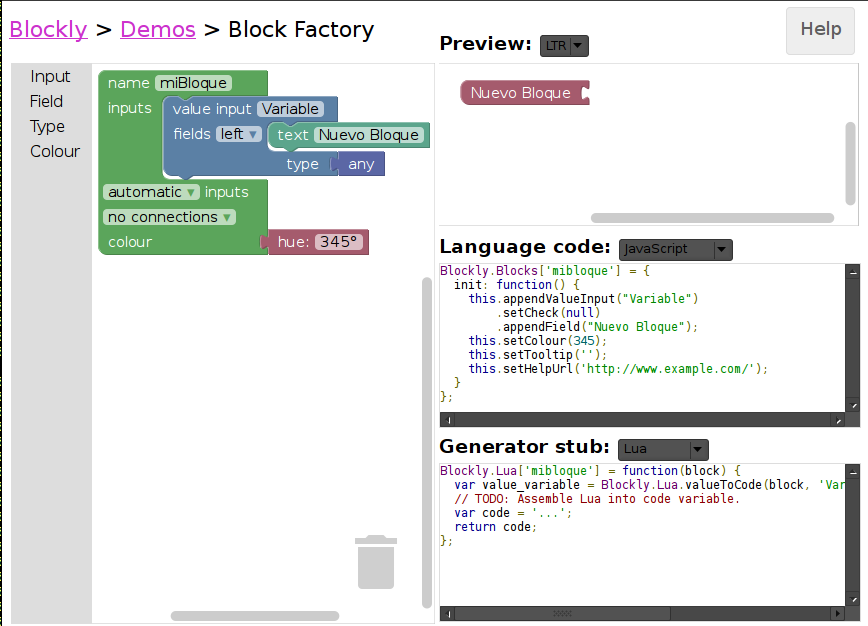
\includegraphics[scale=0.4]{imag/blocklyfactory.png}
    \caption{BlocklyFactory}
    \label{fig:blocklyfactory}
\end{figure}
\smallskip

\twocolumn


\end{document}
